\documentclass[10pt, a4paper]{article}

% GRAPHICS
\usepackage{graphicx}

% FONTS
\usepackage{palatino}
\usepackage[T1]{fontenc}

% PAGE BORDERS
\usepackage[top=40mm, bottom=20mm, left=25mm, right=25mm]{geometry}

% PARAGRAPH BEHAVIOUR
\setlength{\parskip}{1em}
\setlength{\parindent}{0pt}

% VERBATIM INPUT
\usepackage{verbatim}

\author{William Hunter}
\title{ToPy Installation Instructions}

\begin{document}

\begin{figure}[!ht]
\centering

\includegraphics[scale=0.25]{topy_logo3d.png}
\end{figure}

\tableofcontents

\section{What is this document?}
This is really just a PDF version of \texttt{INSTALL.txt} which you'll find in the ToPy zip file.

\section{Where to get ToPy}
If you're reading this, you most probably have it already. But here's the URL in any case:

\texttt{code.google.com/p/topy}.

At the URL above, go to the \textsf{Downloads} tab and download the zip file corresponding to the version
number below under requirements. Unzip and follow the instructions in \texttt{INSTALL.txt} or this document.

ToPy was last tested and worked on \textsf{Windows 7}.

ToPy was originally developed on \textsf{GNU/Linux}
(Ubuntu).

\clearpage
\section{ToPy requirements}
The following is copied (included, actually) verbatim from \texttt{INSTALL.txt}:

\verbatiminput{INSTALL.txt}

\clearpage
\section{Sample ToPy terminal/console output}
In case you don't believe me\ldots
\begin{figure}[!ht]
\centering
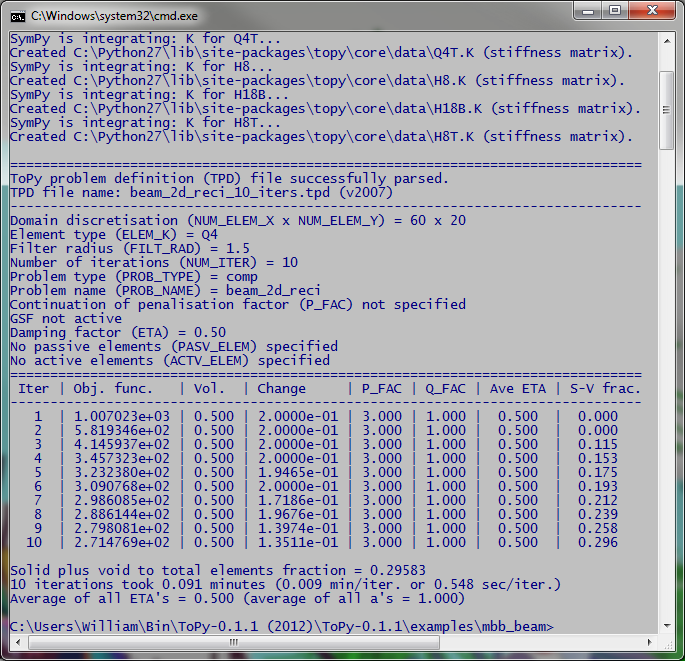
\includegraphics[width=160mm]{CWindowssystem32cmd.png}
\end{figure}


--\\
\textsf{William Hunter}\\
2012-03-04
\end{document}